% ============================================================
%  يُترجَم بـ XeLaTeX  (في Overleaf: Menu → Compiler → XeLaTeX)
%  الخط: Amiri (متوفر في Overleaf، أو حمّله من github.com/aliftype/amiri)
% ============================================================
\documentclass[12pt,a4paper]{article}
\usepackage[a4paper,margin=1.7cm,top=2.3cm,bottom=2.9cm,headheight=15pt,footskip=1.5cm]{geometry}
\usepackage{amsmath,amssymb}
\usepackage{icomma}
\usepackage[english,bidi=default,layout=lists]{babel}
\babelprovide[import,main]{arabic}
\babelfont{rm}[Scale=1.08]{Amiri}
\babelfont{sf}[Scale=1.08]{Amiri}
\usepackage[most]{tcolorbox}
\usepackage{tikz}
\usetikzlibrary{arrows.meta,calc,shadings}
\usepackage{array}
\usepackage{colortbl}
\usepackage{fancyhdr}
\usepackage{titlesec}
\usepackage{enumitem}
\usepackage{collcell}
\usepackage{needspace}
\usepackage{etoolbox}
% أعمدة جداول تُكتب خلاياها بالعربية في الاتجاه الصحيح
\newcolumntype{C}{>{\collectcell\ar}c<{\endcollectcell}}
% تجنب عنوان يتيم في أسفل الصفحة
\pretocmd{\section}{\Needspace{15\baselineskip}}{}{}
\pretocmd{\subsection}{\Needspace{11\baselineskip}}{}{}

% ---------- الألوان ----------
\definecolor{cDef}{HTML}{1F4E9C}
\definecolor{cThm}{HTML}{B3261E}
\definecolor{cRem}{HTML}{2E7D32}
\definecolor{cEx}{HTML}{C76B00}
\definecolor{cMeth}{HTML}{6A1B9A}
\definecolor{cSol}{HTML}{00695C}
\definecolor{cSec}{HTML}{1F3A68}

% ---------- العناوين ----------
\titleformat{\section}{\Large\bfseries\color{cSec}}{\thesection.}{0.6em}{}[{\color{cSec!60}\titlerule[1pt]}]
\titleformat{\subsection}{\large\bfseries\color{cThm!85!black}}{\thesubsection.}{0.5em}{}
\titlespacing*{\section}{0pt}{14pt}{8pt}
\titlespacing*{\subsection}{0pt}{10pt}{5pt}
\setlength{\parindent}{0pt}
\setlength{\parskip}{4pt}
\setlist{itemsep=2pt,topsep=3pt}

% ---------- الصناديق (تُرسم في سياق LTR ويُكتب محتواها بالعربية) ----------
\newtcolorbox{arbox}[3][]{enhanced,
  colback=#2!5,colframe=#2!80!black,arc=2mm,boxrule=0.8pt,
  left=6pt,right=6pt,top=8pt,bottom=5pt,
  fonttitle=\bfseries,coltitle=white,
  title={\foreignlanguage{arabic}{#3}},
  attach boxed title to top right={xshift=-5mm,yshift=-3mm},
  boxed title style={colback=#2!80!black,arc=1.5mm,boxrule=0pt},
  before upper={\selectlanguage{arabic}},
  before skip=8pt,after skip=8pt,breakable,#1}
\newenvironment{BOX}[2]{\begin{otherlanguage}{english}\begin{arbox}{#1}{#2}}{\end{arbox}\end{otherlanguage}}
\newenvironment{tarif}[1][تعريف]{\begin{BOX}{cDef}{#1}}{\end{BOX}}
\newenvironment{khassia}[1][خاصية]{\begin{BOX}{cThm}{#1}}{\end{BOX}}
\newenvironment{molahada}[1][ملاحظة]{\begin{BOX}{cRem}{#1}}{\end{BOX}}
\newenvironment{mithal}[1][مثال]{\begin{BOX}{cEx}{#1}}{\end{BOX}}
\newenvironment{tariqa}[1][طريقة]{\begin{BOX}{cMeth}{#1}}{\end{BOX}}

% ---------- التمارين والحلول ----------
\newcounter{exo}
\newenvironment{tamrin}[1]{\stepcounter{exo}\begin{BOX}{cSec}{التمرين \theexo: #1}}{\end{BOX}}
\newenvironment{hal}{\Needspace{12\baselineskip}\begin{otherlanguage}{english}\begin{arbox}[breakable]{cSol}{حل التمرين \theexo}}{\end{arbox}\end{otherlanguage}}

% رسومات TikZ تُوضع في سياق LTR
\newenvironment{LTR}{\begin{otherlanguage}{english}}{\end{otherlanguage}}
\newcommand{\ar}[1]{\foreignlanguage{arabic}{#1}}

% ---------- رموز ----------
% نقاط الحذف داخل الرياضيات (\dots يسبب خللاً في الاتجاه مع babel)
\renewcommand{\dots}{\mathinner{\ldotp\ldotp\ldotp}}
\renewcommand{\ldots}{\mathinner{\ldotp\ldotp\ldotp}}
\renewcommand{\cdots}{\mathinner{\cdotp\cdotp\cdotp}}
\newcommand{\N}{\mathbb{N}}
\newcommand{\Z}{\mathbb{Z}}
\newcommand{\D}{\mathbb{D}}
\newcommand{\Q}{\mathbb{Q}}
\newcommand{\R}{\mathbb{R}}
\newcommand{\pgcd}{\operatorname{PGCD}}
\newcommand{\ppcm}{\operatorname{PPCM}}

% ---------- تمثيل مجال على مستقيم عددي ----------
% \NLseg{a}{b}{[}{]}  مجال محدود
\newcommand{\NLseg}[4]{\begin{LTR}\begin{tikzpicture}[baseline=-0.6ex]
 \draw[-{Stealth[length=2mm]},gray!70](0,0)--(3.4,0);
 \draw[line width=2pt,cThm!80!black](0.7,0)--(2.7,0);
 \node[cThm!80!black,font=\LARGE] at (0.7,0){$#3$};
 \node[cThm!80!black,font=\LARGE] at (2.7,0){$#4$};
 \node[below=3pt,font=\footnotesize] at (0.7,0){$#1$};
 \node[below=3pt,font=\footnotesize] at (2.7,0){$#2$};
\end{tikzpicture}\end{LTR}}
% \NLright{a}{[}  مجال نحو +∞
\newcommand{\NLright}[2]{\begin{LTR}\begin{tikzpicture}[baseline=-0.6ex]
 \draw[-{Stealth[length=2mm]},gray!70](0,0)--(3.4,0);
 \draw[line width=2pt,cThm!80!black](1.3,0)--(3.3,0);
 \node[cThm!80!black,font=\LARGE] at (1.3,0){$#2$};
 \node[below=3pt,font=\footnotesize] at (1.3,0){$#1$};
\end{tikzpicture}\end{LTR}}
% \NLleft{b}{]}  مجال نحو −∞
\newcommand{\NLleft}[2]{\begin{LTR}\begin{tikzpicture}[baseline=-0.6ex]
 \draw[-{Stealth[length=2mm]},gray!70](0,0)--(3.4,0);
 \draw[line width=2pt,cThm!80!black](0.05,0)--(2.1,0);
 \node[cThm!80!black,font=\LARGE] at (2.1,0){$#2$};
 \node[below=3pt,font=\footnotesize] at (2.1,0){$#1$};
\end{tikzpicture}\end{LTR}}

% ---------- أيقونات مواقع التواصل (مرسومة بـ TikZ، لا تحتاج أي حزمة) ----------
\definecolor{cFB}{HTML}{1877F2}
\definecolor{cTG}{HTML}{229ED9}
\definecolor{cIG1}{HTML}{FEDA75}
\definecolor{cIG2}{HTML}{D62976}
\definecolor{cIG3}{HTML}{4F5BD5}
\newcommand{\fbicon}{\begin{LTR}\begin{tikzpicture}[baseline=-0.75ex,x=1em,y=1em]
 \fill[cFB] (0,0) circle (0.55);
 \node[white,inner sep=0,font=\usefont{TU}{lmss}{bx}{n}\small] at (0.04,-0.02) {f};
\end{tikzpicture}\end{LTR}}
\newcommand{\igicon}{\begin{LTR}
\begin{tikzpicture}[baseline=-0.75ex,x=1em,y=1em]
 \shade[lower left=cIG1,lower right=cIG2,upper left=cIG2,upper right=cIG3,rounded corners=0.28em] (-0.55,-0.55) rectangle (0.55,0.55);
 \draw[white,line width=0.09em,rounded corners=0.18em] (-0.36,-0.36) rectangle (0.36,0.36);
 \draw[white,line width=0.09em] (0,0) circle (0.17);
 \fill[white] (0.22,0.22) circle (0.05);
\end{tikzpicture}\end{LTR}}
\newcommand{\tgicon}{\begin{LTR}
\begin{tikzpicture}[baseline=-0.75ex,x=1em,y=1em]
 \fill[cTG] (0,0) circle (0.55);
 \fill[white] (-0.33,0.0) -- (0.32,0.27) -- (0.2,-0.3) -- (0.0,-0.15) -- (-0.08,-0.28) -- (-0.08,-0.08) -- cycle;
 \fill[cTG!70!black] (-0.08,-0.08) -- (0.25,0.2) -- (0.0,-0.15) -- (-0.08,-0.28) -- cycle;
\end{tikzpicture}\end{LTR}}
% سطر مواقع التواصل أسفل كل صفحة
% (يُكتب السطر بترتيب بصري من اليسار إلى اليمين: الأيقونة يمين كل اسم)
\newcommand{\PageBox}{\begin{LTR}\tikz[baseline=(p.base)]\node[fill=black,text=white,inner sep=2.5pt,minimum width=1.6em,minimum height=1.3em,font=\usefont{TU}{lmss}{bx}{n}\small](p){\ifnum\value{page}<10 0\fi\arabic{page}};\end{LTR}}
\newcommand{\SocialRow}{\begin{otherlanguage}{english}%
 \ar{\textbf{الأستاذ سوايسية هشام للرياضيات}}\ \tgicon\hfill
 \textbf{prof\_hicham\_math}\ \igicon\hfill
 \ar{\textbf{الأستاذ سوايسية هشام للرياضيات}}\ \fbicon\hspace{2.2em}\PageBox\end{otherlanguage}}
% ---------- رأس وتذييل الصفحة ----------
\pagestyle{fancy}
\fancyhf{}
\renewcommand{\headrulewidth}{0.6pt}
\renewcommand{\footrulewidth}{0.4pt}
% \SetHeader{يمين الرأس}{يسار الرأس}{يمين التذييل}{يسار التذييل}
\newcommand{\SetHeader}[2]{%
 \fancyhead[C]{\parbox{\textwidth}{\ar{#1\hfill #2}}}%
 \fancyfoot[C]{\parbox{\textwidth}{\small\SocialRow}}}

\usepackage{tkz-tab}
\usepackage{multicol}
% جدول تغيرات / إشارة (يُرسم في سياق LTR)
\newenvironment{TAB}{\par\begin{center}\begin{LTR}\begin{tikzpicture}[scale=0.95,every node/.style={font=\small}]}{\end{tikzpicture}\end{LTR}\end{center}}
% معلم بشبكة: \begin{GR}{xmin}{xmax}{ymin}{ymax}{unit cm}
\newenvironment{GR}[5]{\par\begin{center}\begin{LTR}\begin{tikzpicture}[x=#5cm,y=#5cm,font=\footnotesize]
 \def\xmn{#1}\def\xmx{#2}\def\ymn{#3}\def\ymx{#4}
 \draw[gray!25,very thin] (#1,#3) grid (#2,#4);
 \draw[-{Stealth[length=2mm]}] (#1,0)--(#2+0.3,0) node[below left]{$x$};
 \draw[-{Stealth[length=2mm]}] (0,#3)--(0,#4+0.3) node[below left]{$y$};
 \node[below left] at (0,0){$O$};
 \draw[very thick,-{Stealth[length=1.6mm]}] (0,0)--(1,0) node[below,pos=.55]{$\vec i$};
 \draw[very thick,-{Stealth[length=1.6mm]}] (0,0)--(0,1) node[left,pos=.55]{$\vec j$};
 \begin{scope}\clip (#1,#3) rectangle (#2,#4);}
{\end{scope}\end{tikzpicture}\end{LTR}\end{center}}
\newcommand{\Ticks}[2]{\foreach \t in {#1} \node[below,font=\scriptsize] at (\t,0){$\t$}; \foreach \t in {#2} \node[left,font=\scriptsize] at (0,\t){$\t$};}
\newcommand{\bx}[1]{\ensuremath{\colorbox{cDef!12}{$\displaystyle #1$}}}
\newcommand{\hl}[1]{\ensuremath{\colorbox{cEx!20}{$\displaystyle #1$}}}
\newcommand{\Lim}[1]{\displaystyle\lim_{x\to #1}}
\newcommand{\Cf}{(C_f)}
\newenvironment{qst}{\begin{enumerate}[label=\protect\circled{\arabic*},leftmargin=*]}{\end{enumerate}}
\newcommand{\circled}[1]{\foreignlanguage{english}{\tikz[baseline=(c.base)]\node[circle,fill=cDef,text=white,inner sep=1.2pt,font=\scriptsize\bfseries](c){#1};}}
% عمودان: \TwoCol{عرض اليسار}{محتوى اليسار}{عرض اليمين}{محتوى اليمين}  (آمن مع TikZ)
\newcommand{\TwoCol}[4]{\par\begin{LTR}\noindent\begin{minipage}[t]{#1\textwidth}\selectlanguage{arabic}#2\end{minipage}\hfill\begin{minipage}[t]{#3\textwidth}\selectlanguage{arabic}#4\end{minipage}\end{LTR}\par}
\newcommand{\un}{(u_n)}\newcommand{\vn}{(v_n)}
% برهان بالتراجع: \Rec{الخاصية P(n)}{التحقق من P(0)}{البرهان على الوراثة}
\newcommand{\Rec}[3]{\textbf{برهان بالتراجع:} نسمي $P(n)$ الخاصية: «#1».
\begin{itemize}
\item \textbf{التحقق:} #2
\item \textbf{الوراثة:} نفرض أن $P(n)$ صحيحة ونبرهن صحة $P(n+1)$: #3
\item \textbf{الخلاصة:} حسب مبدأ الاستدلال بالتراجع، $P(n)$ صحيحة من أجل كل عدد طبيعي $n$.
\end{itemize}}
\newcommand{\src}[1]{{\footnotesize\textbf{#1}}\par}
\newcommand{\ok}{$\textcolor{cRem}{\checkmark}$}
\newcommand{\limn}{\displaystyle\lim_{n\to+\infty}}
% أسئلة فرعية (أ) (ب) (جـ) كل سؤال في سطر
\newenvironment{sq}{\begin{itemize}[leftmargin=2.4em,itemsep=3pt]}{\end{itemize}}
\newcommand{\qa}{\item[(أ)]}\newcommand{\qb}{\item[(ب)]}\newcommand{\qc}{\item[(جـ)]}\newcommand{\qd}{\item[(د)]}\newcommand{\qe}{\item[(هـ)]}
\newcommand{\pa}{\par\smallskip\textbf{(أ)} }\newcommand{\pb}{\par\smallskip\textbf{(ب)} }\newcommand{\pc}{\par\smallskip\textbf{(جـ)} }\newcommand{\pd}{\par\smallskip\textbf{(د)} }\newcommand{\pe}{\par\smallskip\textbf{(هـ)} }
\newcommand{\ccl}[1]{\par\textbf{الخلاصة:} #1}

\pretocmd{\section}{\Needspace{24\baselineskip}}{}{}
\SetHeader{\small\bfseries\color{cSec}تمارين: الدوال المرجعية}{\small\color{cSec}السنة الأولى ثانوي -- جذع مشترك علوم وتكنولوجيا}
\begin{document}
\newcolumntype{M}[1]{>{\centering\arraybackslash}p{#1}}
\newcommand{\RL}[4]{\TwoCol{#3}{#4}{#1}{#2}}
\newcommand{\QQ}[1]{\par\smallskip\textbf{#1.} }
\newcommand{\ABC}[3]{\\[2pt]\begin{tabular}{p{0.28\textwidth}p{0.28\textwidth}p{0.28\textwidth}}(جـ) \ #3 & (ب) \ #2 & (أ) \ #1\end{tabular}}
\newcommand{\cp}[2]{\begin{pmatrix}#1\\#2\end{pmatrix}}
\newcommand{\V}[1]{\overrightarrow{#1}}
\newcommand{\Ax}[4]{\draw[gray!22] (#1,#3) grid (#2,#4);
\draw[->] (#1-0.2,0)--(#2+0.3,0) node[right]{$x$}; \draw[->] (0,#3-0.2)--(0,#4+0.3) node[above]{$y$};
\foreach \t in {#1,...,#2} {\ifnum\t=0\else\node[below,font=\tiny] at (\t,0){$\t$};\fi}
\foreach \t in {#3,...,#4} {\ifnum\t=0\else\node[left,font=\tiny] at (0,\t){$\t$};\fi}
\node[below left,font=\tiny] at (0,0){$O$};}
\begin{LTR}
\begin{tcolorbox}[enhanced,colback=cSec,colframe=cSec,arc=3mm,halign=center,boxrule=0pt,top=12pt,bottom=12pt,before upper={\selectlanguage{arabic}}]
{\color{white}\fontsize{26}{32}\selectfont\bfseries سلسلة تمارين: الدوال المرجعية}\\[8pt]
{\color{white}\large تمارين متنوعة ونماذج اختبارات -- بدون حلول (للتدرّب) والتمثيلات البيانية}\\[5pt]
{\color{white}\large السنة الأولى ثانوي -- جذع مشترك علوم وتكنولوجيا}
\end{tcolorbox}
\end{LTR}

% =====================================================================
\section{الدالة «مربع» والدوال كثيرات الحدود من الدرجة الثانية}
% ------------------------------------------------- 1
\begin{tamrin}{الشكل النموذجي ودالة تآلفية}
$f$ الدالة المعرّفة على $\R$ بـ: $f(x)=x^2+2x-1$ ، و $(C)$ تمثيلها البياني في معلم متعامد ومتجانس $(O;\vec i,\vec j)$.
\begin{enumerate}
\item بيّن أنه يمكن كتابة $f(x)$ على الشكل $f(x)=(x+a)^2+b$ ، مع تعيين $a$ و $b$.
\item ادرس اتجاه تغير الدالة $f$ على المجالين $]-\infty;-1]$ و $[-1;+\infty[$.
\item شكّل جدول تغيرات الدالة $f$ ، ثم استنتج القيمة الحدية للدالة $f$ وبيّن نوعها.
\item ارسم المنحنى $(C)$ اعتماداً على التمثيل البياني للدالة مربع.
\item لتكن $g$ الدالة التآلفية المعرّفة على $\R$ حيث $g(-2)=-1$ و $g(1)=2$.
\begin{sq}
\qa أعط عبارة $g(x)$.
\qb ارسم التمثيل البياني لـ $g$ في نفس المعلم السابق.
\qc حل بيانياً ثم جبرياً في $\R$: \ $f(x)=g(x)$ و $f(x)>g(x)$.
\end{sq}
\end{enumerate}
\end{tamrin}

% ------------------------------------------------- 2
\begin{tamrin}{دراسة شاملة لدالة من الدرجة الثانية}
$h$ الدالة المعرّفة بـ: $h(x)=x^2-6x+3$ ، و $(C_h)$ تمثيلها البياني في معلم متعامد ومتجانس.
\begin{enumerate}
\item جد مجموعة تعريف الدالة $h$ ، ثم احسب صور الأعداد $-2$ ، $0$ و $1$.
\item تحقق أنه من أجل كل عدد حقيقي $x$: \ $h(x)=(x-3)^2-6$.
\item احسب السوابق الممكنة للأعداد $3$ ، $-2$ و $-5$.
\item ادرس اتجاه تغير $h$ على $]-\infty;3]$ و $[3;+\infty[$ ، ثم شكّل جدول تغيراتها.
\item تحقق أن $h(x)+6\ge0$ من أجل كل $x$. ماذا يمثل العدد $-6$ بالنسبة للدالة $h$؟
\item عيّن نقطة تقاطع $(C_h)$ مع محور التراتيب.
\item هل يمكن رسم $(C_h)$ انطلاقاً من منحنى الدالة المرجعية $x\mapsto x^2$؟ علّل ، ثم ارسمه.
\item انطلاقاً من $(C_h)$ ، ما هي شفعية الدالة $h$؟
\end{enumerate}
\end{tamrin}

% ------------------------------------------------- 3
\begin{tamrin}{دالة معرّفة بجدول تغيراتها ودالة من الدرجة الثانية}
\textbf{I.} إليك جدول تغيرات دالة $f$ معرّفة على المجال $[-5;3]$:
\begin{TAB}
\tkzTabInit[lgt=1.3,espcl=2.2]{$x$/0.7,$f(x)$/1.6}{$-5$,$-2$,$0$,$3$}
\tkzTabVar{-/$-1$,+/$4$,-/$-2$,+/$2$}
\end{TAB}
\begin{enumerate}
\item عيّن القيمتين الحديتين الكبرى والصغرى للدالة $f$ على $[-5;3]$.
\item قارن مع التبرير بين العددين $f(-1)$ و $f\Big(-\dfrac12\Big)$ ، ثم بين $f(2)$ و $f(3)$.
\item ماذا يمكنك القول عن شفعية الدالة $f$؟
\item ماذا يمكن قوله عن عدد حلول المعادلة $f(x)=0$؟ شكّل جدول إشارة $f$.
\item أنشئ تمثيلاً بيانياً تقريبياً للدالة $f$.
\end{enumerate}
\textbf{II.} $g$ الدالة المعرّفة على $\R$ بـ: $g(x)=x^2+4x+3$.
\begin{enumerate}
\item تحقق أنه من أجل كل $x$: $g(x)=(x+3)(x+1)$ و $g(x)=(x+2)^2-1$.
\item احسب صور الأعداد $0$ ، $\sqrt3$ و $-2$.
\item باستعمال العبارة المناسبة ، أوجد السوابق الممكنة للعددين $0$ و $3$.
\item ادرس اتجاه تغير $g$ ، ثم اشرح كيف يمكن استنتاج منحناها $(C)$ من منحنى الدالة مربع ، ثم أنشئهما.
\end{enumerate}
\end{tamrin}

% ------------------------------------------------- 4
\begin{tamrin}{وضعية إدماجية: تقليص التكاليف}
\RL{0.55}{%
تريد إحدى المؤسسات صنع «رمز» له الشكل المقابل (وحدة الأطوال هي السنتيمتر): مستطيل $CDEF$ يعلوه مثلث $ABG$ ، حيث $BG=60$ ، والارتفاع الكلي $40$ ، و $BC=FG=x$ ، وارتفاع المثلث $2x$.\par
وقصد تقليص التكاليف نبحث عن قيمة $x$ التي تكون من أجلها مساحة الشكل أصغر ما يمكن.}{0.42}{%
\begin{LTR}\centering
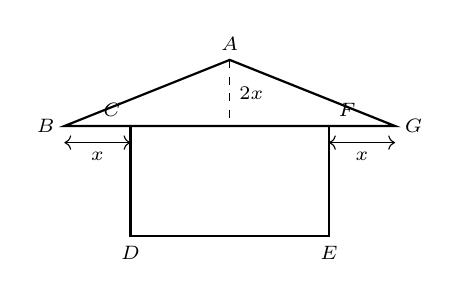
\begin{tikzpicture}[scale=0.07,font=\scriptsize]
\draw[thick] (0,20)--(30,32)--(60,20)--cycle;
\draw[thick] (12,20)--(12,0)--(48,0)--(48,20);
\draw[dashed] (30,32)--(30,20);
\node[left] at (0,20){$B$}; \node[above] at (30,32){$A$}; \node[right] at (60,20){$G$};
\node[above left] at (12,20){$C$}; \node[above right] at (48,20){$F$}; \node[below] at (12,0){$D$}; \node[below] at (48,0){$E$};
\draw[<->] (0,17)--(12,17) node[midway,below]{$x$}; \draw[<->] (48,17)--(60,17) node[midway,below]{$x$};
\node[right] at (30,26){$2x$};
\end{tikzpicture}
\end{LTR}}
\begin{enumerate}
\item عبّر بدلالة $x$ عن: الطولين $CF$ و $CD$ ، ثم مساحة المستطيل $CDEF$ ومساحة المثلث $ABG$.
\item استنتج أن مساحة الشكل هي: $4x^2-140x+2400$.
\item نعتبر الدالة $f$ المعرّفة على $[0;20]$ بـ: $f(x)=4x^2-140x+2400$.
\begin{sq}
\qa اكتب الشكل النموذجي لـ $f(x)$.
\qb ادرس اتجاه تغير $f$ على كل من المجالين $\Big[0;\dfrac{35}2\Big]$ و $\Big[\dfrac{35}2;20\Big]$ ، ثم شكّل جدول تغيراتها.
\qc استنتج قيمة $x$ التي تكون من أجلها مساحة الشكل أصغر ما يمكن ، وحدد هذه المساحة.
\end{sq}
\end{enumerate}
\end{tamrin}

% =====================================================================
\section{الدالة «مقلوب» والدوال الكسرية}
% ------------------------------------------------- 5
\begin{tamrin}{دالة كسرية من الشكل $k+\dfrac1{x+c}$}
$f$ الدالة المعرّفة على $\R-\{-2\}$ بـ: $f(x)=\dfrac{2x+5}{x+2}$ ، و $(C_f)$ تمثيلها البياني في معلم متعامد ومتجانس.
\begin{enumerate}
\item بيّن أنه من أجل كل عدد حقيقي $x\ne-2$: \ $f(x)=2+\dfrac1{x+2}$.
\item ادرس اتجاه تغير $f$ على المجالين $]-\infty;-2[$ و $]-2;+\infty[$ ، ثم شكّل جدول تغيراتها.
\item بيّن أن النقطة $A(-1;3)$ تنتمي إلى $(C_f)$.
\item ليكن $(P)$ التمثيل البياني للدالة مقلوب. اشرح كيف يمكن إنشاء $(C_f)$ انطلاقاً من $(P)$ ، ثم أنشئه.
\end{enumerate}
\end{tamrin}

% ------------------------------------------------- 6
\begin{tamrin}{تعيين وسيطين ونقط التقاطع مع المحورين}
$f$ دالة معرّفة على $\R-\{1\}$ بـ: $f(x)=\dfrac{2x-1}{x-1}$ ، و $(C_f)$ تمثيلها البياني في معلم متعامد ومتجانس.
\begin{enumerate}
\item عيّن العددين الحقيقيين $a$ و $b$ بحيث من أجل كل $x\ne1$: $f(x)=a+\dfrac{b}{x-1}$.
\item ادرس اتجاه تغير $f$ على المجالين $]-\infty;1[$ و $]1;+\infty[$ ، ثم شكّل جدول تغيراتها.
\item عيّن نقط تقاطع $(C_f)$ مع محوري الإحداثيات.
\item بيّن أنه يمكن استنتاج $(C_f)$ انطلاقاً من التمثيل البياني للدالة مقلوب ، ثم أنشئ $(C_f)$.
\end{enumerate}
\end{tamrin}

% ------------------------------------------------- 7
\begin{tamrin}{دالتان: مربع ومقلوب مع متراجحة}
لتكن الدالتان $f$ و $g$ المعرّفتان بـ: $f(x)=x^2+bx+\dfrac14$ و $g(x)=\dfrac{-2x-1}{x+1}$ ، حيث $b$ عدد حقيقي ، و $(C_f)$ ، $(C_g)$ تمثيلاهما في معلم متعامد ومتجانس.
\begin{enumerate}
\item أوجد قيمة $b$ حتى تقبل المعادلة $f(x)=0$ حلاً مضاعفاً ، ثم أوجد هذا الحل.
\item نضع $b=1$.
\begin{sq}
\qa تحقق أن الشكل النموذجي لـ $f(x)$ هو $\Big(x+\dfrac12\Big)^2$ ، ثم حل باستعمال التحليل المعادلة: $f(x)-(3x-1)(2x+1)=0$.
\qb حل في $\R$ المعادلة $x^2+2x-3=0$ ، ثم استنتج حلول المتراجحة: $\dfrac{x\,f(x)}{x^2+2x-3}\le0$.
\qc حل المعادلة $\sin^2x+2\sin x-3=0$ حيث $x$ ينتمي إلى المجال $[0;\pi]$.
\end{sq}
\item ادرس اتجاه تغير $f$ على المجالين $\Big]-\infty;-\dfrac12\Big]$ و $\Big[-\dfrac12;+\infty\Big[$ ، ثم شكّل جدول تغيراتها واستنتج القيمة الحدية لها.
\item
\begin{sq}
\qa تحقق أن $g(x)=-2+\dfrac1{x+1}$ ، ثم ادرس اتجاه تغير $g$ على $]-\infty;-1[$ و $]-1;+\infty[$.
\qb عيّن نقط تقاطع $(C_g)$ مع محوري الإحداثيات.
\end{sq}
\item
\begin{sq}
\qa بيّن كيف يمكن رسم $(C_f)$ و $(C_g)$ ، ثم ارسمهما في نفس المعلم.
\qb حل بيانياً المتراجحة $g(x)-f(x)\le0$.
\end{sq}
\end{enumerate}
\end{tamrin}

% =====================================================================
\section{الدائرة المثلثية ، الجيب وجيب التمام}
% ------------------------------------------------- 8
\begin{tamrin}{تحويل وتمثيل على الدائرة المثلثية}
\begin{enumerate}
\item حوّل إلى الراديان قيس الزاوية $140^\circ$ ، ثم $210^\circ$ ، وإلى الدرجة قيس الزاوية $-\dfrac{3\pi}5$ ، ثم $\dfrac{15\pi}{4}\,rad$.
\item عيّن على الدائرة المثلثية $(C)$ النقط $A$ ، $B$ ، $C$ و $D$ صور الأعداد:
\[\frac{2023\pi}{3}\quad;\quad\frac{1447\pi}{4}\quad;\quad-125\pi\quad;\quad\frac{7\pi}6.\]
\item عيّن جيب وجيب تمام كل عدد من الأعداد السابقة.
\end{enumerate}
\end{tamrin}

% ------------------------------------------------- 9
\begin{tamrin}{حساب الجيب من جيب التمام والعكس}
\begin{enumerate}
\item احسب $\sin x$ إذا علمت أن $\cos x=-\dfrac{\sqrt3}2$ و $x\in\,]-\pi;0[$.
\item احسب $\cos x$ إذا علمت أن $\sin x=\dfrac12$ و $x\in\Big[0;\dfrac\pi2\Big[$.
\item احسب $\cos x$ إذا علمت أن $\sin x=\dfrac35$ و $x\in\Big[\dfrac\pi2;\pi\Big]$.
\item نضع $\cos x=-\dfrac35$ حيث $x\in\Big[\dfrac\pi2;\pi\Big]$. \ احسب $\sin x$ ، ثم $\cos(\pi-x)+\sin(2\pi-x)$.
\end{enumerate}
\end{tamrin}

% ------------------------------------------------- 10
\begin{tamrin}{تبسيط عبارات مثلثية}
\begin{enumerate}
\item $x$ عدد حقيقي ، نضع: $A(x)=2\sin(\pi-x)+\cos(\pi+x)-2\sin\Big(\dfrac{2023\pi}{3}+\pi\Big)-\cos\Big(\dfrac{-1444\pi}{4}+x\Big)$.
\begin{sq}
\qa بيّن أن: $A(x)=2\sin x+\sqrt3$.
\qb حل في المجال $]-\pi;\pi]$ المعادلة $A(x)=0$.
\end{sq}
\item $E(x)=-\cos(-x+92\pi)-\sin(-x+15\pi)+\sin(x+9\pi)-\cos\Big(\pi+\dfrac\pi3\Big)$. \ بسّط العبارة $E(x)$ ، ثم احسب $E(0)$ و $E\Big(\dfrac\pi2\Big)$.
\item $B(x)=\cos\Big(\dfrac{17\pi}2\Big)+\sin(2019\pi+x)-\cos(x+11\pi)$.
\begin{sq}
\qa أثبت أن $B(x)=\cos x-\sin x$.
\qb احسب $B(x)$ من أجل $x=-\dfrac\pi4$.
\qc أثبت أنه من أجل كل $x$: $\big[B(x)\big]^2=1-2\cos x\sin x$ ، ثم احسب $\Big[B\Big(\dfrac{2020\pi}{4}\Big)\Big]^{2020}$.
\end{sq}
\end{enumerate}
\end{tamrin}

% ------------------------------------------------- 11
\begin{tamrin}{قيم مضبوطة ومتطابقات}
\begin{enumerate}
\item حوّل إلى الراديان $47^\circ$ ، وإلى الدرجة $\dfrac{3\pi}7\,rad$.
\item
\begin{sq}
\qa إذا علمت أن $\cos\dfrac\pi5=\dfrac{\sqrt5+1}4$ ، بيّن أن $\sin\dfrac\pi5=\dfrac{\sqrt{10-2\sqrt5}}4$.
\qb استنتج القيم المضبوطة لكل من: $\sin\Big(-\dfrac{6\pi}5\Big)$ ، $\cos\Big(\dfrac{11\pi}5\Big)$ و $\tan\dfrac\pi5$.
\end{sq}
\item عيّن قيم $x$ من المجال $[0;\pi]$ في الحالتين: (أ) $\cos x=\dfrac{\sqrt2}2$ \quad (ب) $\sin x=\dfrac12$.
\item بيّن أنه من أجل كل عدد حقيقي $x$:
\begin{sq}
\qa $(\sin x+\cos x)^2=1+2\sin x\cos x$
\qb $(1+\sin x+\cos x)^2=2(1+\cos x)(1+\sin x)$
\qc $1+\tan^2x=\dfrac1{\cos^2x}$ \ (حيث $\cos x\ne0$)
\qd $\dfrac1{\tan^2x}-\cos^2x=\dfrac{\cos^2x}{\tan^2x}$ \ (حيث $x\in\,]0;\frac\pi2[$)
\end{sq}
\end{enumerate}
\end{tamrin}

% =====================================================================
\section{اختيار من متعدد ، صحيح أم خطأ}
% ------------------------------------------------- 12
\begin{tamrin}{اختيار من متعدد}
لكل حالة اقتراح واحد صحيح ، اختره مع التبرير:
\begin{enumerate}
\item الزاوية $a=\dfrac{7\pi}{12}\,rad$ يقابلها:
\ABC{$105^\circ$}{$90^\circ$}{$135^\circ$}
\item $\cos\Big(\dfrac{2017\pi}6\Big)$ يساوي:
\ABC{$-\dfrac{\sqrt3}2$}{$\dfrac12$}{$\dfrac{\sqrt3}2$}
\item $A(x)=\cos(\pi+x)+\sin(\pi-x)+\cos(-x)$ تساوي:
\ABC{$\cos x$}{$0$}{$\sin x$}
\item الدالة $f(x)=\cos x\times\sin x$:
\ABC{فردية}{زوجية}{لا فردية ولا زوجية}
\item $\cos\Big(\dfrac{2023\pi}4\Big)$ يساوي:
\ABC{$\dfrac{\sqrt2}2$}{$-\dfrac{\sqrt2}2$}{$\dfrac12$}
\item إذا كان $\cos x=-\dfrac45$ و $x\in\Big[\pi;\dfrac{3\pi}2\Big]$ فإن $\sin x$ يساوي:
\ABC{$-\dfrac54$}{$-\dfrac35$}{$\dfrac45$}
\item $f$ دالة تآلفية حيث $f(0)=-2$ و $f(2)=8$. عبارتها:
\ABC{$-5x-2$}{$-5x+2$}{$5x-2$}
\item الدالة $x\mapsto\dfrac1x$ على المجال $]0;+\infty[$:
\ABC{متزايدة}{متناقصة}{غير رتيبة}
\end{enumerate}
\end{tamrin}

% ------------------------------------------------- 13
\begin{tamrin}{صحيح أم خطأ}
أجب بصحيح أو خطأ مع التعليل:
\begin{enumerate}
\item منحنى الدالة $f:x\mapsto\sqrt{x+1}-2$ هو صورة منحنى الدالة جذر تربيعي بالانسحاب الذي شعاعه $\vec u\cp{-1}{2}$.
\item المستقيم الذي يشمل النقطة $A\Big(\dfrac12;\dfrac32\Big)$ و $\vec v\cp13$ شعاع توجيه له معادلته: $3x-y=0$.
\item الدالة $g:x\mapsto\dfrac{2-3x}{2x}$ المعرّفة على $\R^*$ متزايدة تماماً على $]0;+\infty[$.
\item إذا كان $0<x<1$ فإن $x^2<x$.
\item من أجل كل عدد حقيقي $x$: $\sqrt{x^2}=x$.
\item الدالة مكعب متزايدة تماماً على $\R$.
\item منحنى الدالة $x\mapsto(x-3)^2+1$ رأسه النقطة $S(-3;1)$.
\end{enumerate}
\end{tamrin}

\end{document}
